\documentclass[letterpaper,titlepage,12pt,oneside,spanish,final]{report_eie}

%\documentclass[letterpaper,titlepage,12pt,twoside,openright,spanish,final]{report_eie}

%%%%%%%%%%%%%%%%%%%%%%%%%%%%%%%%%%%%%%%%%%%%%%%%%%%%%%%%%%%%%%%%%%%%%%%%
\usepackage[spanish]{babel}
\usepackage[utf8]{inputenc}
\usepackage[T1]{fontenc}  %Estilo de fuente time new roman

\usepackage{amssymb}
\usepackage{amsfonts}
\usepackage{amsmath}
\usepackage{latexsym}
\usepackage[letterpaper]{geometry}

\usepackage{float}
\usepackage{makeidx}
\usepackage{color}

\usepackage{tocbibind}
\usepackage{acronym}
\usepackage{epsfig}
\usepackage{graphicx}
\usepackage{setspace}
\usepackage{multicol}
\usepackage{longtable}
%\usepackage{doublespace}
\usepackage[document]{ragged2e}
\usepackage{fancyhdr}
%\usepackage{fancyheadings}
\usepackage{indentfirst}
\usepackage{booktabs}

%========= Define el estilo de referencias ===============
%\usepackage[round,authoryear]{natbib}%\usepackage[square,numbers]{natbib}%
%\usepackage[comma,authoryear]{natbib} esto está abajo

%========= Define el estilo de referencias IEEE ===============
%in the preamble
\usepackage[
backend=biber,
style=ieee,
citestyle=numeric
]{biblatex}

\addbibresource{referencias.bib} %Imports bibliography file
\usepackage{csquotes}
\usepackage[compact]{titlesec} %modificar espaciado


\usepackage{url}
\usepackage{hyperref}
%\usepackage[dvips,colorlinks=true,urlcolor=red,citecolor=black,anchorcolor=black,linkcolor=black]{hyperref}
%%%%%%%%%%%%%%%%%%%%%%%%%%%%%%%%%%%%%%%%%%%%%%%%%%%%%%%%%%%%%%%%%%
%            Definición del Documento PDF, (PDFLaTeX)            %
%%%%%%%%%%%%%%%%%%%%%%%%%%%%%%%%%%%%%%%%%%%%%%%%%%%%%%%%%%%%%%%%%%

\hypersetup{pdfauthor=Guillermo Raven}

\hypersetup{pdftitle=Trabajo Especial de Grado}%

\hypersetup{pdfkeywords=Robot manipulador}

\pdfstringdef{\Produce}{Escuela de Ingeniería Eléctrica, Facultad de Ingeniería, UCV}%

\pdfstringdef{\area}{Área del trabajo}

\hypersetup{pdfproducer=\Produce}

\hypersetup{pdfsubject=\area}

\hypersetup{bookmarksnumbered=true}

%%%%%%%%%%%%%%%%%%%%%%%%%%%%%%%%%%%%%%%%%%%%%%%%%%%%%%%%%%%%%%%%%%
%\setcounter{MaxMatrixCols}{10}


%===================== Re-definición de Ambientes =================
\newtheorem{theorem}{Teorema}
\newtheorem{acknowledgement}[theorem]{Acknowledgement}
\newtheorem{algoritmo}[theorem]{Algorithm}
\newtheorem{supuestos}[theorem]{Supuestos}
\newtheorem{hipotesis}[theorem]{Hipótesis}
\newtheorem{axiom}[theorem]{Axiom}
\newtheorem{case}[theorem]{Case}
\newtheorem{claim}[theorem]{Claim}
\newtheorem{conclusion}[theorem]{Conclusión}
\newtheorem{condition}{Condición}
\newtheorem{conjecture}{Conjecture}
\newtheorem{corollary}{Corollary}
\newtheorem{criterion}{Criterion}
\newtheorem{definition}{Definición}  %{Definition}
\newtheorem{example}[theorem]{Ejemplo}%{Example}
\newtheorem{exercise}[theorem]{Exercise}
\newtheorem{lemma}{Lemma}
\newtheorem{notation}[theorem]{Notation}
\newtheorem{problem}{Problem}
\newtheorem{property}{Property}
\newtheorem{proposition}{Proposition}
\newtheorem{remark}[theorem]{Remark}
\newtheorem{solution}{Solution}
\newtheorem{summary}[theorem]{Summary}
\newenvironment{proof}[1][Proof]{\noindent\textbf{#1.} }{\ \rule{0.5em}{0.5em}}%

\numberwithin{equation}{chapter}%
\numberwithin{figure}{chapter}%
\numberwithin{table}{chapter}%
\numberwithin{definition}{chapter}%
\numberwithin{lemma}{chapter}%
\numberwithin{theorem}{chapter}%
\numberwithin{corollary}{chapter}%
\numberwithin{condition}{chapter}%
\numberwithin{criterion}{chapter}%
 \numberwithin{problem}{chapter}%
\numberwithin{property}{chapter}%
\numberwithin{proposition}{chapter}%
\numberwithin{solution}{chapter}%
\numberwithin{conjecture}{chapter}%

%==================== Separación en sílabas ========================
\hyphenpenalty=6800%

%A
\hyphenation{a-pro-xi-ma-do}


%B
\hyphenation{ba-lan-ce}%

%C
\hyphenation{co-la-bo-ra-do-res}%
\hyphenation{co-rres-pon-dien-tes}%
\hyphenation{co-rres-pon-dien-te}%
\hyphenation{con-ti-nua-men-te}%
\hyphenation{con-si-de-ra-cio-nes}%
\hyphenation{cons-tru-ir}%
\hyphenation{con-si-de-ra-do}%


%D
\hyphenation{di-fe-ren-cia}%
\hyphenation{des-cri-tos}%
\hyphenation{dis-mi-nu-ye}%
\hyphenation{des-cri-to}%
\hyphenation{de-pen-dien-tes}%


%E
\hyphenation{ex-pe-ri-men-to}
\hyphenation{ex-pe-ri-men-ta-cion} %


%P
\hyphenation{pro-ba-bi-li-da-des}%
\hyphenation{pro-ba-bi-li-dad}%
\hyphenation{par-ti-cu-lar}%

%M
\hyphenation{mo-da-li-da-des}%
\hyphenation{mo-de-lo} %
\hyphenation{me-dian-te}%
 \hyphenation{man-te-ni-mien-tos}%
%N

%O
\hyphenation{ope-ra-cio-nal}%
\hyphenation{o-pe-ra-cion}%
\hyphenation{o-pe-ra-cio-nes} %
\hyphenation{o-pe-ra-do-ra}%

%==================== Diseño de Página =============================
%\pagestyle{headings}
%\setlength{\headheight}{0.2cm}
\setlength{\textwidth}{14.52cm}%
%\pagestyle{fancy}
%\renewcommand{\sectionmark}[1]{\markright{\thesection\ #1}}
%\rhead[\fancyplain{}{\bfseries\thepage}]{\fancyplain{}{\bfseries\rightmark}}%\thepage
%\lhead[\fancyplain{}{\bfseries\leftmark}]{\fancyplain{}{\bfseries}} \cfoot{}%

%\fancyhead[R]{}


\rfoot[\fancyplain{}{\textit{E. Brea}}] {\fancyplain{}{}}
\lfoot[\fancyplain{}{}] {\fancyplain{}{\textit{}}}    %%%%%%%%%%%%%%%%%%% OJO ACA %%%%%%%%%%
\cfoot[\fancyplain{}{}] {\fancyplain{}{\bfseries\thepage}}
%\setlength{\footrulewidth}{0.0pt}%
%\setlength{\headrulewidth}{0.1pt}%

%===================================================================



%================== Diseño de Párrafo y delimitador ================
\renewcommand{\baselinestretch}{1.5}% Espaciado entre linea
\geometry{left=4cm,right=3cm,top=3cm,bottom=3cm}
\frenchspacing %
%\raggedright % Sólo para justificar el texto a la izquierda
\setlength{\parindent}{0.7cm}% Espacio de la sangría
\setlength{\parskip}{14pt plus 1pt minus 1pt}% Separación entre párrafos

%\setlength{\parskip}{1ex plus 0.5ex minus 0.2ex}%

%==========================  Español venezolano =====================
%%Personalización de caption
\addto\captionsspanish{%
  \def\prefacename{Prefacio}%
  \def\refname{REFERENCIAS}%
  \def\abstractname{Resumen}%
  \def\bibname{REFERENCIAS}%{Bibliografía}%
  \def\chaptername{CAPÍTULO}%
  \def\appendixname{Apéndice}%{Anexo}
  \def\contentsname{ÍNDICE GENERAL}
  \def\listfigurename{LISTA DE FIGURAS}%Índice de Figuras\hspace*{10em}
  \def\listfigurenameTofC{LISTA DE FIGURAS}%Índice de Figuras
  \def\listtablename{LISTA DE TABLAS}%Índice de Tablas
  \def\indexname{Índice alfabético}%
  \def\figurename{Figura}%
  \def\tablename{Tabla}%
  \def\partname{Parte}%
  \def\enclname{Adjunto}%
  \def\ccname{Copia a}%
  \def\headtoname{A}%
  \def\pagename{Página}%
  \def\seename{véase}%
  \def\alsoname{véase también}%
  \def\proofname{Demostración}%
  \def\glossaryname{Glosario}
  }%



%==================================================================

%\setcounter{secnumdepth}{1}
%\setcounter{page}{4}
%\addtocounter{page}{4}%

\pagenumbering{roman}

\makeindex



%%%%%%%%%%%%%%%%%%%%%%%%%%%%%%%%%%%%%%%%%%%%%%%%%%%%%%%%%%%%%%%%%

\begin{document}
%\frontmatter
%===================================================================
%                            Primera Página
%================================== Portada =================================================
\renewcommand{\baselinestretch}{1.0}% Espaciado entre linea
\begin{center}
\huge{\textbf{Anteproyecto}}\\
\vspace{5cm}
\large{\textbf{DESARROLLO DE UN PAQUETE EN PYTHON PARA EL POSICIONAMIENTO DE OBJETOS EN UNA ESCENA MEDIANTE VISIÓN ESTEREOSCÓPICA Y TÉCNICAS DE RECONOCIMIENTO BASADAS EN APRENDIZAJE AUTOMÁTICO
 }}
\vspace{0.5cm}
\\
Br. Guillermo Raven\\
Dpto. Electrónica, Computación y Control\\
Escuela de Ingeniería Eléctrica,
Facultad de Ingeniería\\
Universidad Central de Venezuela\\
\end{center}
\vspace{0.8cm}

\begin{flushleft}
\begin{spacing}{1}
    %TUTOR ACADÉMICO: Profesora Tamara Pérez\\
   % TUTOR INDUSTRIAL: Ingeniero Carlos Rodríguez
\end{spacing}
\end{flushleft}
\justifying
\chapter*{INTRODUCCIÓN}\label{CAP:intro}
\setlength{\parskip}{14pt}% Separación entre párrafos
\addcontentsline{toc}{chapter}{INTRODUCCIÓN}%
%\markboth{Introducción}{Introducción}%

\pagenumbering{arabic}%
Se entiende por posicionamiento en el campo de visión por computador (VC) a todas aquellas técnicas que permiten extraer las coordenadas espaciales de un objeto a partir de su representación en 2 dimensiones. Entre las técnicas empleadas para el posicionamiento, aquellas que utilizan visión estéreo son ampliamente utilizadas en el campo de la robótica y los vehículos autónomos. Este hecho no es de extrañar, debido a que los inicios de esta tecnología datan de 1838 cuando Sir Charles Wheatstone publico un articulo en el que describía la visión estereoscópica \cite{Wheatstone1837}, en dicho articulo explica el como esta tecnología se basaba en la visión humana y en la separación de, aproximadamente, 65 mm que existe entre nuestros ojos. Estos reciben cada uno una imagen diferente que el cerebro une creando el efecto de tridimensionalidad. Por supuesto no tardo mucho hasta que decidieron aplicar esta teoría en el invento de moda de la época, las cámaras, y hoy en día el camino que se ha recorrido para permitir que un computador pueda interpretar coordenadas espaciales de una imagen nos ha permitido emplear las cámaras como sensores que interpretan el entorno que les rodea. 

En robótica se han desarrollado diversas metodologías de control basadas en sensores que dotan al robot de sentidos para percibir el mundo que le rodea. Algunas de las técnicas más usadas en el entorno industrial dependen de la odometría, que no es mas que el estudio de  la estimación de la posición de vehículos con ruedas durante la navegación. Para realizar esta estimación se usa información sobre la rotación de las ruedas mediante encoders con el fin de estimar cambios en la posición a lo largo del tiempo. Por otro lado, las técnicas de visión por computador en las décadas recientes, se han vuelto cada vez mas importantes debido al incremento en la capacidad de procesamiento y almacenamiento de los dispositivos electrónicos, además de la creciente necesidad realizar tareas más complejas con los autómatas, son flexibles a tal punto de que pueden ser implementadas con una o varias cámaras, las imágenes captadas son preprocesadas mediante filtros y luego con algoritmos, es posible determinar que objetos se encuentran en la imagen. Si se emplean metodologías basadas en visión estéreo, cámaras RGBD o láser, el robot gana la capacidad de localizarse en el entorno de trabajo o localizar objetos respecto al mismo.

En la actualidad las técnicas mas avanzadas de visión por computador (VC) utilizan las abstracciones conocidas como redes neuronales artificiales (RNA), las cuales suelen ser programadas en frameworks OpenSource basados en python, orientados al aprendizaje automático (AA). Algunos de los mas populares son Tensorflow o Keras por su compatibilidad con dispositivos embebidos  e incluso OpenCV para el preprocesamiento de las imágenes. Estas redes son capaces de aprender patrones en conjuntos de datos que se le suministra y dependiendo de como se le entrene pueden generalizar para datos que no se encuentren en el conjunto de datos de entrenamiento. En el campo de VC se traduce en detectar objetos para obtener la localización del mismo en una imagen o clasificar el tipo de objeto.

En la industria Venezolana no son muy comunes desarrollos en el campo de la localización de objetos en una escena, por lo que las técnicas de visión para el control no son muy comunes, de modo que las estrategias de control de robots suelen basarse en odometría o fusión de sensores, sumados a un conjunto de restricciones e instrucciones que controlen el movimiento de los autómatas. Por este motivo se propone desarrollar un paquete en Python que permita a programadores e ingenieros implementar sistemas de control cuya data sean imágenes provenientes de escenas estereoscópicas, los cuales podrán ser implementados en robots de uso domestico e industrial.

\section*{Planteamiento del problema}
Las técnicas de control y automatización de procesos, aplicadas en el campo de la robótica, permiten realizar tareas sencillas en entornos estructurados donde se conoce el espacio de trabajo por completo y los objetos que interactúan en el mismo. No obstante, hoy en día los autómatas son capaces de realizar tareas complejas en espacios de trabajo dinámicos, es decir, entornos que varían en el tiempo, donde los eventos son de carácter estocástico. Sin embargo, para lograr dicha proeza es necesario expandir el conjunto de técnicas de control convencionales mediante la incorporación de nuevos algoritmos y estrategias.  

Para resolver problemas de robótica en entornos complejos, las mejores estrategias actuales son aquellas que dotan al robot de la capacidad de aprender y adaptarse a los cambios, estas técnicas de inteligencia artificial requieren de información del entorno la cual es extraída mediante algoritmos de VC que otorgan al autómata la habilidad de reconocer los objetos en su campo de visión y a partir de imágenes en 2D captar las posiciones relativas entre los objetos de interés y el robot. 

Existen diversas formas de conocer las posiciones de de objetos en escenas, una de ellas es la visión estéreo, aunque su implementación puede ser complicada si no se poseen los conocimientos apropiados, por este motivo se busca desarrollar un paquete que facilite la implementación de técnicas de posicionamiento de objetos en escenas mediante visión estéreo y reconocimiento basado en AA.
\section*{Justificación}
El paquete para el posicionamiento basado en reconocimiento, facilitara la implementación de estrategias de control que empleen visión por computador a ingenieros y programadores. Y servirá para la comprensión de algunas de las técnicas de VC implementadas mediante tecnologías Open Source, como lo son Tensorflow, Keras y OpenCV.

Además de establecer algunos métodos para fortalecer los conocimientos en el área de control  que se imparten en la Escuela de Ingeniería Eléctrica, el estudio de tecnologías que se encuentran en auge usadas en el campo de inteligencia artificial aplicada a la robótica. 
\section*{Antecedentes}
En primer lugar se tiene el trabajo de fin de máster presentado en 2010 por
Martín Montalvo Martínez en la Universidad computense de Madrid, titulado "Técnicas de visión estereoscópica para determinar la estructura tridimensional de la escena"  \cite{MartinMM}.

En este trabajo se estudió la efectividad de diversos métodos de correspondencia estereoscópica, las técnicas utilizadas fueron comparadas mediante un estimador conocido como Error Cuadrático Medio (ECM), con este estimador se comparó el mapa de disparidad obtenido con cada uno de los métodos y el mapa de disparidad considerado como correcto "ground-truth". 
\\
El estudio se centro en la factibilidad para la implementación de sistemas estereoscópicos que han de operar en el exterior y bajo condiciones adversas, ya que las actividades de investigación planteadas por el grupo ISCAR en 2010 estaban orientadas en la navegación autónoma de vehículos. En estos vehículos el principal problema era el de la correspondencia estereoscópica, por este motivo el proyecto se oriento en la identificación de un algoritmo apropiado para el caso correspondiente.
\\
\\
La metodología empleada por el autor consistió en primer lugar, en realizar una revisión bibliográfica sobre los métodos descritos hasta la fecha, luego selecciono aquellos que encajaran con la problemática de estudio, para posteriormente implementarlos en el entorno de Matlab en su versión 2007b utilizando imágenes sintéticas y reales de las que poseía información sobre los mapas de disparidad. Luego evaluó su efectividad mediante el ECM y se obtuvo que de los métodos estudiados el que presenta mejores resultados es aquel basado en la segmentación y medida de similitud, además dicho método  se posiciona como el segundo más rápido al evaluar el promedio de tiempo. Sin embargo el problema que plantea radica en que los objetos existentes en la escena con una tonalidad uniforme y con distintos valores de disparidad son representados incorrectamente en el mapa final. Con este trabajo de maestría se logro comparar el comportamiento de varias metodologías que permiten obtener una representación tridimensional de una escena mediante visión estéreo.
\\
\\
En octubre Dembys, Gao, Shafiekhani, y Desouza (2019) presentaron un paper en una conferencia titulado "Detección de objetos y estimación de pose utilizando CNN (Convolutional Neural Networks) en hardware integrado para tecnología de asistencia" \cite{AssistiveTech}.
\\
\\
En este trabajo se desarrollo un algoritmo de visión estéreo el cual puede ser ejecutado en una placa Raspberry Pi 3 utilizando dos camaras RPi V2 como sensores. Este sistema se interconecta a un computador mediante el framework ROS (Robot Operating System) el cual posee una interfaz donde muestra el resultado final del sistema estereoscópico. El algoritmo utilizado esta compuesto por dos fases principales, la primera sería la fase de detección donde emplea una red neuronal convolucional (CNN) llamada MobileNet SSD (Single Shot MultiBox Descriptor) para reconocer y seguir los objetos de interés en una escena, mientras que en la fase de estimación de posición emplea correspondencias estéreo para reconstruir en 3D las coordenadas espaciales basadas en el algoritmo ORB (Oriented FAST and Rotated BRIEF) desarrollado por OpenCV. La motivación de esta investigación fue el desarrollo de equipamiento médico de bajo coste que pueda servir de apoyo para personas con discapacidades.
\\
\\
Los investigadores compararon sus resultados con la tecnología del estado del arte DOPE (Deep Object Pose Estimation) y llegaron a la conclusión de que es posible integrar redes ligeras para la detección de objetos en tiempo real y estimación de pose en tecnologías de asistencia a un bajo costo. Sin embargo, el algoritmo propuesto depende de la iluminación de la escena y la calidad de las características extraídas del objeto de destino, aunque los resultados demuestran que su enfoque también puede ser empleado en tareas de pick-and-place de brazos manipuladores.
\section*{Objetivos}
\subsection*{Objetivo general}
Desarrollar un paquete en Python para el posicionamiento de objetos en una escena empleando visión estereoscópica y técnicas de reconocimiento basadas en aprendizaje automático.
\subsection*{Objetivo especifico}
\begin{itemize}
    \item Describir al menos dos técnicas de reconocimiento basadas en aprendizaje automático empleadas en el posicionamiento de objetos.
    \item Realizar el análisis de requerimientos necesarios del software a desarrollar.
    \item Definir la arquitectura del software.
    \item Definir los patrones de diseño aplicables.
    \item Seleccionar el modelo de aprendizaje automático para el reconocimiento de imágenes en vídeo.
    \item Implementar el sistema de reconocimiento con Tensorflow/Keras y OpenCV, en el lenguaje de programación Python.
    \item Implementar un algoritmo para el posicionamiento, basado en el reconocimiento de objetos en la escena.
    \item Diseñar un banco de pruebas para la validación del paquete.
    \item Elaborar un documento descriptivo del paquete con ejemplos de uso.
    \item Empaquetar el software para su distribución o instalación.
\end{itemize}
\section*{Metodología}
Para la elaboración de este trabajo se seccionarán los conjuntos de tareas a realizar en 10 etapas:
\subsection*{Etapa 1: Documentación}
En esta etapa se investigaran a profundidad los fundamentos de los algoritmos de reconocimiento basados en AA, los pasos necesarios para permitir la visión estéreo y las estrategias utilizadas al momento de desarrollar paquetes en Python.
\subsection*{Etapa 2: Análisis de requerimientos, construcción y diseño del soporte físico para el sistema de adquisición de data}
Utilizando los fundamentos aprendidos se analizaran los requerimientos del software a desarrollar y partir de ellos se realizaran los esquemas de una estructura de soporte para las cámaras de teléfonos, dicha estructura debe permitir reajustar la distancia entre cámaras de ser necesario. Una vez diseñada, se utilizarán materiales reciclables para su construcción.
\subsection*{Etapa 3: Definir la arquitectura del software}
Se realizara un diagrama donde se organicen los elementos necesarios para el funcionamiento del paquete, subdividiendo las partes del mismo en módulos independientes. Se definirán las pautas para la documentación del mismo, la forma en la que se realizaran las pruebas unitarias y se seleccionara el paquete que se empleara para permitir la posterior distribución.
\subsection*{Etapa 4: Definir los patrones de diseño aplicables}
Con los módulos subdivididos, se establecerán los patrones de diseño adecuados para cada modulo tomando en cuenta la relación existente entre los mismos. Esto permitirá la reutilización de código en los casos que se requiera resolver problemas recurrentes en el paquete.
\subsection*{Etapa 5: Seleccionar el modelo de aprendizaje automático para el reconocimiento de imágenes en vídeo}
De acuerdo con los métodos de reconocimientos estudiados en la etapa 1, se compararan los mismos para luego seleccionar el más adecuado, tomando en cuenta el software y hardware a disposición del autor.
\subsection*{Etapa 6: Desarrollo del o los módulos de reconocimiento de objetos}
Utilizando modelos pre-entrenados, se procederá a diseñar el o los módulos que permitan implementar un sistema de reconocimiento de objetos en una escena. Luego se elaborará un algoritmo que implemente las funciones o métodos contenidos en el modulo o los módulos para el reconocimiento, posteriormente se comprobará la eficacia de los modelos, comparándolos con imágenes de un conjunto de datos o "dataset".
\subsection*{Etapa 7: Desarrollo de los módulos de visión estéreo}
Se programaran para que puedan ser compatibles con los de reconocimiento o puedan implementarse sin utilizar el reconocimiento, de este modo podrá obtenerse un mapa de disparidad de toda la escena sin necesidad de requerir el modulo de reconocimiento, esto agrega flexibilidad en cuanto a funciones del paquete. Luego se elaborara un algoritmo que implemente las funciones o métodos contenidos en los módulos y posteriormente se comprobara el funcionamiento mediante un dataset de imágenes RGBD.
\subsection*{Etapa 8: Elaboración del banco de pruebas}
En todo el desarrollo del software, se realizaran pruebas unitarias que permitan comprobar el funcionamiento independiente de los módulos ante diferentes entradas de datos. Y cuando todos los módulos sean completados se realizaran pruebas generales que permitan comprobar el correcto funcionamiento del paquete.
\subsection*{Etapa 9: Creación de documento descriptivo}
Empleando el paquete o los paquetes para la documentación seleccionados en la etapa 3, se desarrollara un documento descriptivo auto generado por python que permita ilustrar al usuario sobre la correcta utilización del software desarrollado. 
\subsection*{Etapa 10: Distribución del paquete}
Por último se procederá a empaquetar el software para su distribución.
\section*{Alcance y limitaciones}
El presente trabajo estará acotado en el desarrollo del paquete para el posicionamiento de objetos, en un entorno cerrado con la iluminación adecuada, para el correcto funcionamiento del modulo de reconocimiento. Se realizaran pruebas mediante cámaras de teléfono cuyos datos serán enviados a través de la aplicación gratuita de android IP webcam, para luego ser procesados en un computador o en un dispositivo embebido.
\section*{Herramientas y equipos a utilizar}
Se poseen los siguientes elementos para la ejecución de este trabajo:
\begin{itemize}
    \item Una laptop.
    \item Dos cámaras de teléfono
    \item La aplicación IP webcam para el envío del par de imágenes de entrada al computador mediante red LAN.
    \item Acceso a un servidor para el procesamiento en caso de requerir una mejor GPU.
\end{itemize}
\section*{Análisis de factibilidad}
Para la realización de este trabajo se cuenta con la documentación necesaria, además de casos de estudio donde lograron implementar sistemas similares en computadores y microcontroladores de gama baja y media. En caso de requerir la potencia de procesamiento que ofrece un servidor en la nube, se tiene un internet estable. El autor ya posee cierto nivel de conocimiento en las áreas de visión por computador y aprendizaje automático. Por otro lado se cuenta con el apoyo del ingeniero Carlos Gonzalez el cual se comprometió en prestar ayuda en el área de aprendizaje automático mediante el framework Tensorflow/Keras.

De ser necesaria alguna otra herramienta o equipo el autor cubrirá los gastos. Y la cantidad de tiempo que se propone se considera suficiente para la realización de este trabajo.
\section*{Cronograma}
En la siguiente Figura se observa la distribución de las etapas en  número de semanas:
\begin{figure}[H]
    \centering
    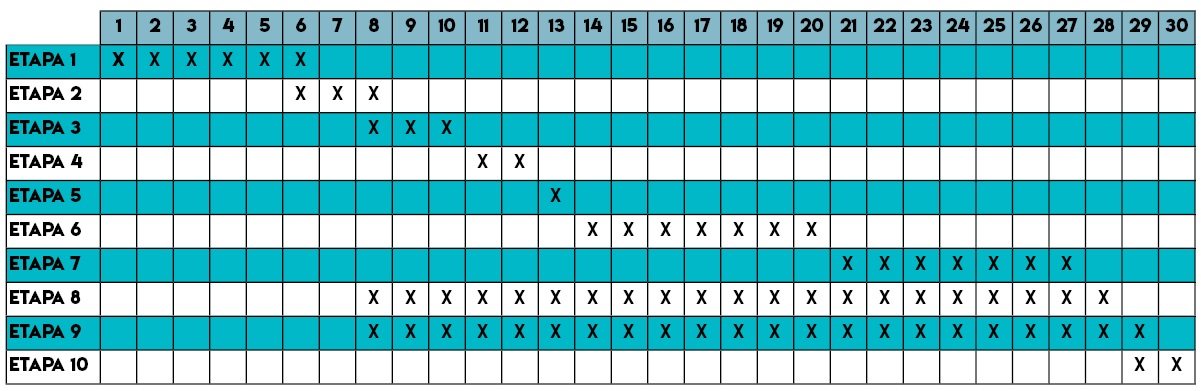
\includegraphics[scale=0.5]{Anteproyecto/cronograma.jpg}
    \caption{Cronograma de actividades}
    \label{cronograma}
\end{figure}

%% No cite
%\markboth{Referencias}{Referencias}%
%\addcontentsline{toc}{chapter}{Referencias}%
\newpage

\printbibliography[title={REFERENCIAS}]

\begin{refsection}[biblioteca.bib]
    \printbibliography[title={BIBLIOGRAFÍA}]
    \nocite{*}
\end{refsection}



% CASE 2: BiBTeX used to generate EIETdeG.bbl (to be further fine tuned)
%\input{EIETdeG.bbl} % outcomment this line in Case


%==================================================================
%\markboth{index}{index}%
%\addcontentsline{toc}{chapter}{Índice alfabético}%
\printindex%

\end{document}